\documentclass[12pt ,a4paper ]{article}

\usepackage[utf8]{inputenc}
\usepackage[T1]{fontenc}      % caractères français
\usepackage[francais]{babel}  %langue
\usepackage[left=2.3cm,right=2.5cm,bottom=2.5cm,top=2.3cm]{geometry}   % marges
\usepackage{verbatim}
\usepackage{float}
\usepackage{graphicx}         % images
\usepackage{verbatim}
\usepackage{multicol}
\usepackage{titlesec}


                           
\begin{document}
	\begin{titlepage}
		
		\vspace{0.5cm}
		\begin{center}		
			{\Large  Master 1 Informatique}
		\end{center}
		\vspace{1cm}
		
		\rule{1\linewidth}{1.1pt}\newline   %regle
		\begin{center}
			 {\Huge \textbf{Rapport de Projet : Traitement Automatique du Texte en IA}}
		\end{center}
		\rule{1\linewidth}{1.1pt} \\
		
		\begin{center}
		\begin{LARGE}
		\textbf{Sujet :} \\\vspace{0.6cm} Identification des opinions exprimées dans les avis et commentaires d’un ordinateur.
		\end{LARGE}
		\end{center}
		
		\vspace{0.5cm}
		\begin{center}	
				\begin{Large}
				Yann MARTIN D'ESCRIENNE \\ 
				Yohann TOGNETTI \\ 
				\end{Large}
		\end{center}
		\vspace{6cm}
		
		\begin{center}
			{\large « Année universitaire 2020 - 2021 »}
		\end{center}
		

\end{titlepage}

\newpage
\tableofcontents 
				
\newpage


\begin{multicols}{2} 
\section{Introduction}

	\subsection{Présentation générale du projet}
		Dans le cadre de notre cours de Traitement automatique du texte en IA, il nous a été demandé d'effectuer un projet de notre choix impliquant une intelligence artificielle travaillant sur des données textuelles. La restriction sur le sujet se limitant à l'existence d'un jeu de données conséquent.
	
	\subsection{Choix du sujet}
		Notre choix de sujet fut \textbf{l'identification des opinions exprimées dans les avis et commentaires d’un ordinateur.} Plus précisément, comment retrouver parmi un ensemble de commentaires les parties de l'ordinateur visées,  sur quels aspects et quel en est l'avis général qui en ressort. 
		
\section{Description des tâches}
Ce sujet est fortement inspiré du "SemEval-2015 Task 12" sur la partie "Aspect Based Sentiment Analysis (ABSA): Laptop Reviews" et partage donc le même objectifs avec des simplifications. Les différentes entités et catégories qui vont suivre provienne également des annotations du sujet de SemEval. Chacun des commentaires est fragmentés phrase par phrase afin de faciliter le travail de l'IA. 
		
\subsection{Entités}
\noindent Tout d'abord il s'agit de retrouver dans la phrase le(s) entité(s) ciblée. Elles peuvent être l'ordinateur comme un tout, ses parties physique (clavier, écran..) , des logiciels ou OS (Windows, navigateur, jeux...) ou bien même une compagnie et ses services. (DELL, Apple, le support technique, la livraison..).\\

\noindent\textit{Remarque : } Rien n'interdit d'avoir plusieurs entités dans la même phrase.\\
		
\noindent Voici la liste des entités possible : 
\begin{itemize}
\item DISPLAY (=moniteur, écran), 
\item CPU (=processeur), 
\item MOTHERBOARD (=carte mère),
\item HARDDISC (=disque dur), 
\item MEMORY (=mémoire, RAM), 
\item BATTERY (=batterie), 
\item POWER\_SUPPLY (=chargeur, unité de chargement, cordon d'alimentation, (power) adapteur),
\item KEYBOARD (=touche, clavier, pavé numérique), 
\item MOUSE (=sourie, pavé tactile)
\item FANS\_COOLING (=ventilateur, système de refroidissement), 
\item OPTICAL\_DRIVES (=lecteur CD, DVD ou Blue-ray),
\item PORTS (=USB, HDMI, VGA, lecteur de carte),
\item GRAPHICS (=carte graphique, carte video),
\item MULTIMEDIA\_DEVICES (=son, audio, microphone, webcam, haut-parleur, casque, écouteurs).
\end{itemize}				

\subsection{Catégories}
\noindent Une fois obtenue il faut également trouver sur quelle(s) catégorie(s) de l'entité le commentaire porte. Cela peut être un aspect général , sa prise en main, ses performances, son design et ses fonctionnalités, etc... \\

\noindent\textit{Remarque : }Là encore, rien n'interdit d'aborder plusieurs catégorie pour la même entité au sein d'une même phrase.\\

\noindent Voici la liste des catégories possible : 
\begin{itemize}
\item GENERAL, 
\item PRICE (=prix), 
\item QUALITY (=qualité), 
\item DESIGN\_FEATURES (=design et fonctionnalités),
\item OPERATION\_PERFORMANCE, 
\item USABILITY (=ergonomie, prise en main), 
\item PORTABILITY (=portabilité),
\item CONNECTIVITY (=connectivité), 
\item MISCELLANEOUS (=divers).
\end{itemize}	

\paragraph{} 
\noindent L'entité E et la catégorie C qui s'y rapporte forme ainsi un couple E\#C. \\

\noindent\textit{Remarque : }Il est à noter la possibilité qu'aucun couple E\#C ne se rapporte à une phrase d'un commentaire.

\subsection{Polarité}
Enfin, chaque phrase (et non chaque couple E\#C comme dans le sujet de SemEval) se verra attribuer une polarité. Les valeurs de cette polarité sont : \textbf{negative} pour les phrases soulignant des défauts ou de mauvais avis, \textbf{positive} pour celles qui au contraire mettent en valeur des points ou des avis positif, \textbf{neutral} lorsque la phrase ne met pas d'opinion en avant et donne par exemple un conseil et finalement \textbf{mixed} pour les textes critiquant un aspect de l'ordinateur mais appréciant un autre. 

\section{Jeux de données}
Les jeux de données se divisent en deux groupes : le jeu de données d'entrée correspondant à ce que l'IA va utiliser pour s'entrainer et celui de test sur lequel les mesures seront effectuées. Tout deux proviennent du site du SemEval. 

\subsection{Structure des jeux de données}
\noindent Ce sont tout deux des documents XML possédant la structure suivante (simplifiée) :  

\begin{figure}[H]
\begin{center}
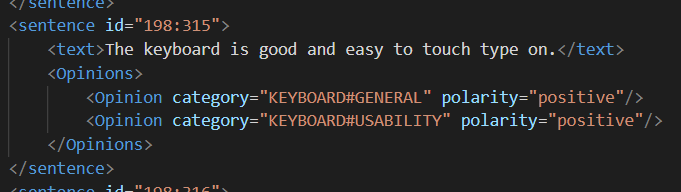
\includegraphics[scale=0.55]{xml_struct.png}
\caption{\small{structure du fichier XML}}
\end{center}
\end{figure}

\subsection{Modification des jeux de données}
Suite à notre implémentation de notre IA qui sera décrite dans le chapitre suivant, de nombreux problèmes nous ont forcés à ajouter nous même des phrases dans le jeu de données d'entrainement.\\

En effet notre IA répond de la présence ou non de chaque couple E\#C dans la phrase actuelle pour chaque combinaison d'entité E et catégorie C. Cela se traduit par une nécessité de nombreuses données appartenant à chacun des couples pouvant apparaitre afin d'obtenir une fonction d'évaluation optimale. 

\paragraph{}
\noindent Environ 350 phrases ont été ajoutées, toutes sont la section 'sentences' d'\textbf{ID 198}. Certaines proviennent d'avis de consommateur sur les ordinateur portables les plus commentés sur Amazon (en anglais), notamment pour les phrases portant sur les clavier, écran, pavé tactile et batterie. Nous avons rédigés le reste pour les catégories plus complexe et moins abordées en générale. Par exemple la qualité des lecteurs DVD ou bien l'ergonomie des OS. \\ 

\noindent \textit{Remarque : } Il est à noté que certain couple n'apparaissent ni dans les données d'entrainement, ni dans les données de test. Par simplification, ces couples ont été ignorés et aucunes phrases n'est étiquetées avec.

\end{multicols}
\end{document}